% -------------------------------------------------------------------- %
% -------------------------------------------------------------------- %
% -------------------------------------------------------------------- %
%\documentclass[10pt]{elsarticle} % here we use the article class, %rather than elsarticle

\documentclass[twocolumn,10pt]{article}

\usepackage[utf8]{inputenc}
\usepackage[T1]{fontenc}
\usepackage{csquotes}
\usepackage[english]{babel}
\usepackage{textcomp}
\usepackage{siunitx}
\usepackage{multicol}
\usepackage[normalem]{ulem}

% -------------------------------------------------------------------- %
% -------------------------------------------------------------------- %
% -------------------------------------------------------------------- %

\usepackage[square,numbers,sort&compress,comma]{natbib}

\sisetup{group-separator={,},
     detect-all,
     binary-units,
     list-units = single,
     range-units = single,
     range-phrase = --,
     per-mode = symbol-or-fraction,
     separate-uncertainty = true,
     multi-part-units = single,
     list-final-separator = {, and },
}
\DeclareSIUnit\atm{atm}
\DeclareSIUnit\bar{bar}

\usepackage{amsmath}
\usepackage{amssymb}
\usepackage{caption}
\usepackage{graphicx}
\usepackage{latexsym}
\usepackage{booktabs}
\usepackage{times}
% packages used for subfigures
\usepackage{caption}
\usepackage{subcaption}
% For including other paper documents
\usepackage{standalone}
% My shortcuts for this document
\usepackage{symposium-styles} % <- My own definitions, not symposium styles

% -------------------------------------------------------------------- %
% -------------------------------------------------------------------- %
% -------------------------------------------------------------------- %

\topmargin - 12pt % might need to be set to 0pt for some installations
\oddsidemargin 32pt
\textheight 610pt
\textwidth 408pt
\columnsep 24pt

% -------------------------------------------------------------------- %
% -------------------------------------------------------------------- %
% -------------------------------------------------------------------- %

\def\thepage{}

\renewenvironment{abstract}%
              {% - begin definition
               \small% - select font
               {\bfseries \abstractname}% - select font
               \par% - end a paragraph (skip \parsep)
               \vspace{10pt}% - add vertical space
              }% - complete definition

\renewcommand\abstractname{Abstract}

\newcommand{\nomenclature}% - name of command
              [1]% - number of arguments
              {% - begin definition
               \bgroup% - begin a local group
               \flushleft% - turn on flushleft option
               \small\bf% - select font
               #1% - insert title text
               \par% - end a paragraph (skip \parsep)
               \egroup% - terminate local group
              }% - complete definition

\renewcommand{\section}% - name of command
              [1]% - number of arguments
              {% - begin definition
               \bgroup% - begin a local group
               \flushleft% - turn on flushleft option
               \small\bf% - select font
               \stepcounter{section}% - increment counter
               \arabic{section}. #1% - insert title text
               \par% - end a paragraph (skip \parsep)
               \egroup% - terminate local group
              }% - complete definition

\renewcommand{\subsection}% - name of command
              [1]% - number of arguments
              {% - begin definition
               \bgroup% - begin a local group
               \flushleft% - turn on flushleft option
               \small\em% - select font
               \stepcounter{subsection}% - increment counter
               \arabic{section}.% - insert title text
               \arabic{subsection}. #1% - insert title text
               \par% - end a paragraph (skip \parsep)
               \egroup% - terminate local group
              }% - complete definition

\renewcommand{\subsubsection}% - name of command
              [1]% - number of arguments
              {% - begin definition
               \bgroup% - begin a local group
               \flushleft% - turn on flushleft option
               \small\em% - select font
               \stepcounter{subsubsection}% - increment counter
               \arabic{section}.% - insert title text
               \arabic{subsection}.% - insert title text
               \arabic{subsubsection}. #1% - insert title text
               \par% - end a paragraph (skip \parsep)
               \egroup% - terminate local group
              }% - complete definition

  \newcommand{\acknowledgement}% - name of command
              [1]% - number of arguments
              {% - begin definition
               \bgroup% - begin a local group
               \flushleft% - turn on flushleft option
               \small\bf% - select font
               #1% - insert title text
               \par% - end a paragraph (skip \parsep)
               \egroup% - terminate local group
              }% - complete definition

  \newcommand{\sectionbib}% - name of command
              [1]% - number of arguments
              {% - begin definition
               \bgroup% - begin a local group
               \flushleft% - turn on flushleft option
               \small\bf% - select font
               #1% - insert title text
               \par% - end a paragraph (skip \parsep)
               \egroup% - terminate local group
              }% - complete definition

\renewcommand\figurename{Fig.}
\renewcommand{\captionsize}{\footnotesize}
\setlength\abovecaptionskip{0pt}
\setlength\belowcaptionskip{0pt}

\renewcommand\bibsection{\sectionbib{\refname}}

\setlength\bibsep{0pt}

\pagenumbering{arabic}

% For compatibility between papers and thesis these are redefined in thesis
\newcommand{\sectionOne}[1]{\section{#1} \addvspace{10pt}}
\newcommand{\sectionTwo}[1]{\subsection{#1} \addvspace{10pt}}
\newcommand{\sectionThree}[1]{\subsubsection{#1} \addvspace{10pt}}

% -------------------------------------------------------------------- %
% -------------------------------------------------------------------- %
% -------------------------------------------------------------------- %

%Reviewer Colors
\usepackage{xcolor}
\definecolor{revOne}{HTML}{cc0000}
\definecolor{revTwo}{HTML}{cc9900}
\definecolor{revThree}{HTML}{238E23}
\definecolor{editor}{HTML}{0057fa}
\definecolor{generalColor}{HTML}{ff5733}

%\newcommand{\revised}[2]{\textcolor{#2}{#1}}  % add
%\newcommand{\former}[2]{\textcolor{#2}{\sout{#1}}}
\newcommand{\revised}[2]{#1}  % add

\begin{document}

\title{\LARGE Generalized preconditioning for accelerating simulations with large kinetic models}

\author{{\large Anthony S.~Walker$^{a}$, Raymond L.~Speth$^{b}$, and Kyle E.~Niemeyer$^{a}$}\\[10pt]
        {\footnotesize \em $^a$School of Mechanical, Industrial, and Manufacturing Engineering, Oregon State University, Corvallis, Oregon, United States}\\
        {\footnotesize \em $^b$Department of Aeronautics and Astronautics, Massachusetts Institute of Technology, Cambridge, Massachusetts, United States}\\[-5pt]}
\date{}

% -------------------------------------------------------------------- %
% -------------------------------------------------------------------- %
% -------------------------------------------------------------------- %

\small
\baselineskip 10pt

% -------------------------------------------------------------------- %
% -------------------------------------------------------------------- %
% -------------------------------------------------------------------- %

\twocolumn[\begin{@twocolumnfalse}
\vspace{50pt}
\maketitle
\vspace{40pt}
\rule{\textwidth}{0.5pt}
\begin{abstract} % 100 to 300 words.
%
Detailed modeling of the combustion of real transportation fuels and the atmospheric reactions involving their emissions is prohibitively expensive, due to the large size and stiffness of the kinetic models.
Adaptive preconditioning is a method used to reduce the cost of integrating large kinetic models by forming a preconditioner based on an semi-analytical Jacobian matrix, paired with sparse linear algebra procedures.
In this study, we extend this preconditioning method to a more-general mole-based state vector formulation applicable to generic reactor types and combinations.
We tested the scheme using constant-pressure and constant-volume ideal-gas reactor simulations, showing speedup in performance from a factor of 3 up to nearly 4000 times for chemical kinetic models with 55 to 7171 species, in comparison with typical dense solvers.
The method also improves performance by a factor of 1.06 to 21.1, for models larger than 200 species, in comparison with a fully exact, analytical Jacobian used as the preconditioner.
Overall, this method improves performance by up to three orders of magnitude for large kinetic models, and offers benefits for models with more than 100 species.
\end{abstract}
\vspace{10pt}
\parbox{1.0\textwidth}{\footnotesize {\em Keywords:}
Chemical kinetics; Implicit integrators; Sparse matrix; Preconditioner; Ordinary differential equations}
\rule{\textwidth}{0.5pt}
\vspace{10pt}
\end{@twocolumnfalse}]

% -------------------------------------------------------------------- %
% -------------------------------------------------------------------- %
% -------------------------------------------------------------------- %

\clearpage


\sectionOne{Introduction}
% Paragraph about how our society relates to combustion

Combustion remains the driving force behind transportation, critical to the world economy and supply chain.
While a necessity, transportation accounts for substantial amounts of greenhouse gas and pollutant emissions that adversely affect the environment and public health~\cite{van_fan_review_2018, manisalidis_environmental_2020}.
Beyond carbon dioxide, the emissions produced consist of many additional chemical species, including pollutants such as carbon monoxide, volatile organic compounds, sulphur oxides, and nitrogen oxides~\cite{van_fan_review_2018}.
Detailed modeling of the combustion of real transportation fuels and the secondary atmospheric reactions involving their emissions is computationally expensive, due to the large sizes of the kinetic models.
For example, with large kinetic models of secondary organic aerosols containing in excess of 5000 species \cite{li_modeling_2015}.
However, simulating and then mitigating the impact of these emissions requires the ability to model such complex phenomena with great detail over a wide range of length and time scales.

% Paragraph about needed research
Most approaches to including detailed chemistry in large-scale reacting-flow simulations currently use methods that either reduce the size of the model, via skeletal reduction or lumping, or eliminate short timescales to reduce stiffness~\cite{Lu2009, Pepiot2019}.
However, even when combined, these methods may not be sufficient to tackle the extremely large (and ever-growing) size of detailed kinetic models for real-fuel combustion and aerosol formation.
Thus, accommodating large kinetic models in simulations also requires improvements in integration methods.
The ordinary differential equations (ODEs) for chemical kinetics are numerically stiff and require implicit integration schemes, which can be particularly expensive for large models because they typically require factorizing large matrices.
Direct solutions of large linear systems are prohibitively expensive and limit large-scale simulations with operations that scale cubically with number of species in the kinetic model.

% Paragraph about our study
In this study, we extend a preconditioning method developed for constant-volume systems \cite{mcnenly_faster_2015} to more-general problems and implement it in the open-source library \cantera{}~\cite{cantera}.
We apply our extended method on ideal gas, constant-pressure reactor simulations, with the goal of obtaining substantial speed-up.
This method, adaptive preconditioning, uses a semi-analytical Jacobian that makes several simplifications to accelerate its formulation.
Notably, the species-rate partial derivatives neglect third-body efficiencies and pressure dependence, and the
the temperature partial derivatives are approximated with finite differences.
Furthermore, the ``adaptive'' feature of the method prunes non-diagonal values when below a specified threshold to further increase sparsity.

Leveraging sparsity has been a strategy for integrating systems of ODEs for quite some time~\cite{brown_reduced_1989, saad_ilut_1994}.
More recently, these strategies have been applied to combustion applications~\cite{marzouk_embedding_2012} and remain a popular method for improving performance.
Others have used analytical Jacobian matrices in lieu of approximate finite-difference Jacobians, which can improve performance by only calculating non-zero matrix elements.
Perini et al.~\cite{perini_analytical_2012} developed exact and approximate analytical Jacobian formulations for gas kinetics that leverage sparsity, implemented in a tool called \texttt{SpeedCHEM}.
They applied these methods with various integration strategies, including preconditioning and incomplete lower-upper (LU) factorization~\cite{perini_study_2014}.
Later, Perini et al.~\cite{perini_fast_2018} used approximate exponential terms and logarithms to further speed up the integration of kinetic models.
Dijkmans et al.~\cite{dijkmans_gpu_2014} used an analytical Jacobian with in situ adaptive tabulation, coupled with efficient routines on graphics processing unit, to accelerate simulations with detailed chemistry.
Similarly, Niemeyer et al.~\cite{niemeyer_pyjac_2017} developed \texttt{pyJac}, an analytical Jacobian generator for chemical kinetics that provides speed-up over finite-difference Jacobian calculations.
%Liang et al.~\cite{liang_towards_2009} demonstrated a proprietary integrator that leverages species-interaction sparsity.
Anzt et al.~\cite{anzt_preconditioned_2017} leveraged sparsity by considering graphics processing unit-based Jacobi iteration and incomplete factorization preconditioning.
Most recently, Lapointe et al.~\cite{lapointe_sparse_2019, lapointe_computationally-efficient_2020} applied adaptive preconditioning to one-dimensional laminar flame simulations and flamelet calculations.

Here, we extend the adaptive preconditioning method to a generalized formulation using a mole-based state vector that is applicable to generic reactor types and combinations of reactors.
We analyze how differences in the generalized formulation affect the structure of the preconditioner.
To determine the impact of tunable parameters, we calculate ignition delays using both a standard direct solver and the preconditioned method with a range of parameter values and kinetic models, and evaluate the performance benefit of the preconditioned method.
On the basis of these results, we develop recommendations or heuristics for solver and parameter selection and discuss directions for future work.


\sectionOne{Methods}
\label{p1:methods-section}

Nearly all numerical combustion codes integrate chemical kinetics using implicit methods to handle the stiffness.
Schemes based on backwards differentiation formula (BDF) are commonly used; here, we focus on the \cvodes{} solver from the \sundials{} package~\cite{cohen_cvode_1996, hindmarsh_sundials_2005}.
The BDF method in \cvodes{} relies on a nonlinear equation solver based on Newton iteration, which requires several linear iterations per nonlinear step.
We use a left-preconditioned Generalized Minimum Residuals (\gmres{})~\cite{trefethen_numerical_1997} method for the linear iterations, which solves a preconditioned system of linear equations.
The solution of the preconditioned system is determined via an incomplete LU decomposition.

First, we set up the system by defining a state vector of length $\ell = \nspecies + 1$, where $\nspecies$ is the number of chemical species.
We represent this system with the state vector
\begin{equation}
    \S{} = \{T, n_1, n_2, n_3, \cdots, n_{\nspecies}\},\quad\S{}\in\mathbb{R}^\ell \;,
\end{equation}
where $T$ is temperature and $n_i$ is the moles of species $i$.
A general system of governing ODEs is
\begin{equation}
    \label{eq:ode-system}
    \frac{d\S{}}{dt} = \F{t,\S{}} \;,
\end{equation}
where $\F{t,\S{}}$ can be a nonlinear function of $t$ and $\S{}$.

Here, we extend the preconditioning strategy to an ideal-gas, constant-pressure reactor system.
The mole-based species conservation equation for the $i^{th}$ species is
\begin{equation}
    \label{eq:species-cons}
    \frac{dn_i}{dt} = V \dot{\omega}_{i} \;,
\end{equation}
where $\dot{\omega}_{i}$ is the net rate of production.
The mole-based conservation of energy equation is
\begin{equation}
    \label{eq:mole-energy}
    \frac{dT}{dt} = \frac{-\SpecSum{\bar{h}_k\dot{\omega}_k}}{\SpecSum{\conc{n_k} \hat{c}_{p,k}}} = \frac{-\SpecSum{\bar{h}_k\dot{n}_k}}{ \SpecSum{n_k \hat{c}_{p,k}}}\;,
\end{equation}
where $\hat{c}_{p,k}$ and $\bar{h}_k$ are the molar constant-pressure specific heat and enthalpy of species $n_k$, respectively.
The volume of the state fluctuates but it is not necessary that we solve an equation for $\dot{V}$. Instead, we calculate the volume needed to maintain constant-pressure with the ideal gas law:
\begin{equation}
    \label{eq:ideal_gas_law}
    V = \frac{NRT}{P} \;.
\end{equation}


\begin{figure}[htb]
    \centering
    \IntegrationOverview[0.85]{}
    \caption{General procedure of a time step using the preconditioned solver.}
    \label{f:integration_process}
\end{figure}

Figure~\ref{f:integration_process} shows the process of integrating one time step, starting with setting up the preconditioner.
The nonlinear solver then starts to make iterations which requires iterations of the linear solver.
In some cases, the preconditioner is reformed during the nonlinear iterations as necessary.

\sectionTwo{Adaptive preconditioning}
\label{sec:methods-adaptive}

The adaptive preconditioning method originally applied to constant-volume systems
by McNenly et al.~\cite{mcnenly_faster_2015} uses a mass-fraction-based approximate Jacobian matrix, which results in a fully dense system for constant-pressure applications.
While a state vector of the form $(T, Y_i)$ is common, a mole-based system $(T, V, n_i)$ has the advantage of enabling a sparse Jacobian, but with the disadvantage being that the system now contains extensive properties \cite{schwer_upgrading_2002}.
As previously mentioned, for ideal gas constant-pressure systems, we can use the ideal gas law to determine the volume necessary to maintain constant pressure, so it is not necessary to directly integrate an equation for volume.
Accordingly, to generalize adaptive preconditioning, we use a mole-based state vector and Jacobian matrix, $\J{\S{}}$, to develop the preconditioner, $\AP$.
This approximate Jacobian is developed by eliminating elements below a certain threshold, computing finite difference temperature derivatives, and neglecting third-body efficiency and pressure dependence in the analytical derivatives $\frac{\partial \dot{n}_i}{\partial n_j}$.


The approximate Jacobian matrix used in this work is
\begin{equation}
    \J{\S{}} =
    \begin{bmatrix}
        \jacline{\dot{T}}
        \jacline{\dot{n}_{1}}
        \dotsline{}
        \jacline{\dot{n}_{\nspecies}}
    \end{bmatrix} \;.
\end{equation}

%
% ----------------d(n_j)/dT------------------
%
We first consider the derivatives with respect to temperature that are approximated with finite differences.
We generalize them as $\frac{\partial \dot{\eta}}{\partial T}$, where $\eta$ is any state variable and $\epsilon$ is a perturbation, such as machine precision (e.g., \texttt{DBL\_EPSILON} in C++):
\begin{equation}
    \label{eq:temp-dervs}
    \frac{\partial \dot{\eta}}{\partial T} = \frac{\dot{\eta}\big\vert_{T+\sqrt{\epsilon}}-\dot{\eta}\big\vert_{T}}{\sqrt{\epsilon}} \;.
\end{equation}

%
% ----------------d(omega_dot)/dn_j------------------
%
The derivatives of Eq.~\eqref{eq:species-cons}, $\frac{\partial \dot{n}_i}{\partial n_j}$, require looping over the number of species $\nspecies$ and number of reactions $\nreactions$.
Since the preconditioner requires that we use moles, we must also convert any concentration-based terms to moles:
\begin{align}
    \conc{n_j} &= \frac{n_j}{V}\\
    \frac{\partial \conc{n_j}}{\partial n_j} &= \frac{1}{V} \;,
\end{align}
where $V$ is the volume of the system.
The species-to-species partial derivatives used in the preconditioner are then
\begin{equation}
    \label{eq:mole-dervs}
    \frac{\partial \dot{n}_i}{\partial n_j} = \frac{\partial V}{\partial n_j} \dot{\omega}_i + V\frac{\partial \dot{\omega}}{\partial n_j} \;,
\end{equation}
where $\dot{\omega}_i$ is the rate of production of species $i$.
We break down Eq.~\ref{eq:mole-dervs} into components to determine the overall terms in a piece-wise manner.
We first consider the derivative of the rate law with respect to moles:
\begin{align}
    \label{eq:full-spec-spec}
    V \frac{\partial \dot{\omega}_i}{\partial n_j} &= V \frac{\partial \dot{\omega}_i}{\partial \conc{n_j}} \frac{\partial \conc{n_j}}{\partial n_j} \nonumber \\
    &= \ReacSum{\nu_{i,k}b_k\frac{\partial R_k}{\partial \conc{n_j}} + \nu_{i,k}R_k\frac{\partial b_k}{\partial\conc{n_j}}} \;,
\end{align}
where $b_k$ is always one, $\nu$ represents the stoichiometric coefficients, and the volume terms cancel.
Since $b_k$ is always one, $\frac{\partial b_k}{\partial\conc{n_j}}=0$ and Equation~\eqref{eq:full-spec-spec} then simplifies to
\begin{equation}
    \label{eq:spec-spec-derv}
    \frac{\partial \dot{\omega}_i}{\partial n_j} = \ReacSum{\nu_{i,k}\frac{\partial R_k}{\partial \conc{n_j}}} \;.
\end{equation}
We continue to break down the rate of progress derivatives into reactant and product contributions as
\begin{multline}
    \frac{\partial R_k}{\partial\conc{n_j}} = k_{f,k}{v_{k,j}^\prime} \conc{n_j}^{v_{k,j}^\prime-1}\ReactSpecProd{\conc{n_h}^{v_{k,h}^\prime}}\\
    -k_{r,k}v_{k,j}^{\prime\prime}\conc{n_j}^{v_{k,j}^{\prime\prime}-1}\ProdSpecProd{\conc{n_h}^{v_{k,h}^{\prime\prime}}} \;,
\end{multline}
where $k$ is the reaction rate and $\alpha$ and $\beta$ represent reactant and product species for the reaction.
To determine $\frac{\partial V}{\partial n_j} \omega_i$, we start with the ideal gas law, Eq.~\eqref{eq:ideal_gas_law}, and obtain
%\former{the form
%\begin{equation*}
%    V = \frac{NRT}{P} \;.
%\end{equation*}
%We use this relation to obtain
\begin{equation}
    \frac{\partial V}{\partial n_j} = \frac{\partial V}{\partial N}\frac{\partial N}{\partial n_j} = \frac{RT}{P} = \frac{V}{N} \;.
\end{equation}
The final expression is then
\begin{multline}
    \frac{\partial \dot{n}_i}{\partial n_j} = \frac{V}{N} \omega_i + \\
    \ReacSum{\nu_{i,k} k_{f,k}{v_{k,j}^\prime} \conc{n_j}^{v_{k,j}^\prime-1}\ReactSpecProd{\conc{n_h}^{v_{k,h}^\prime}}} + \\
    \ReacSum{-\nu_{i,k} k_{r,k}v_{k,j}^{\prime\prime}\conc{n_j}^{v_{k,j}^{\prime\prime}-1}\ProdSpecProd{\conc{n_h}^{v_{k,h}^{\prime\prime}}}} \;.
\end{multline}
%
% ----------------d(dT/dt)/dn_j------------------
%

The derivatives of temperature with respect to different species, $\frac{\partial\dot{T}}{\partial n_j}$, are from Eq.~\eqref{eq:mole-energy}, where we represent the numerator as $a$ and the denominator as $b$.
We find the derivatives by first applying the quotient rule:
\begin{equation}
    \frac{\partial \dot{T}}{\partial n_j} = \frac{a^\prime b - ab^\prime}{b^2} \;.
\end{equation}
The terms in the former equation are then found as
\begin{equation}
    a^\prime b = -N\hat{c}_p\SpecSum{\bar{h}_k \frac{\partial \dot{n}_k}{\partial n_j}}
\end{equation}
and
\begin{equation}
    a b^\prime = -c_{p,j}\SpecSum{\bar{h}_k \dot{n}_k} \;.
\end{equation}
The $a^\prime b$ term actually contains existing Jacobian elements, so in practice we pre-calculate these elements and reuse them here.
Finally, we combine the two parts into the generalized temperature derivative with respect to species $j$:
\begin{equation}
    \label{eq:temp-species}
    \frac{\partial \dot{T}}{\partial n_j} = \frac{-N\hat{c}_p\SpecSum{\bar{h}_k \frac{\partial \dot{n}_k}{\partial n_j}} + c_{p,j}\SpecSum{\bar{h}_k \dot{n}_k}}{(N\hat{c}_p)^2} \;.
\end{equation}

The preconditioner is then formed as
\begin{equation}
    \AP = I - \gamma \J{\S{}} \;,
\end{equation}
where
\begin{equation}
    \gamma = \Delta t \beta
\end{equation}
and $\beta$ is a coefficient in the BDF formulation used to obtain a particular order.
The final step in $\AP$ formation is removing non-diagonal elements below a threshold value, $\xi$:
\begin{equation}
    \AP[i,j] =
    \begin{cases}
        0 & \AP[i,j] < \xi \text{ and } i \neq j, \\
        \AP[i,j] & i = j \text{ or } \AP[i,j] \geq \xi\;.
    \end{cases}
\end{equation}

\begin{table*}[ht] \small
    \centering
    \begin{tabular}{@{}llllll@{}}
        \toprule
        Model & Formula\slash fuel name(s) & Species & Reactions & $\xi_p$ & $\xi_v$\\
        \midrule
        Hydrogen~\cite{smith_gri-mech_1999} & \ce{H2} & 10 & 29 & $10^{-3}$  & $10^{-2}$\\
        GRI-Mech 3.0~\cite{smith_gri-mech_1999} & \ce{CH4} & 55 & 325 & $10^{-3}$ & $10^{-12}$\\
        DME-Propane~\cite{dames_detailed_2016} & \ce{CH3OCH3} \& \ce{C3H8} & 122 & 711 & $10^{-3}$ & $10^{-7}$\\
        HyChem Jet-A~\cite{wang_physics-based_2018, xu_physics-based_2018} & POSF 10325 (\ce{C11H22}) & 203 & 1589 & $10^{-2}$ & $10^{-1}$\\
        Butane~\cite{zhang_shock_2013} & \ce{C4H10} & 230 & 2461 & $10^{-18}$ & $10^{-10}$\\
        2-Butonane~\cite{hemken_2017} & \ce{C4H8O1}-2 & 315 & 1803 & $10^{-1}$ & $10^{-11}$\\
        Isobutene~\cite{li_2016} & \textit{i-}\ce{C4H8} & 493 & 2716 & $10^{-7}$ & $10^{-18}$\\
        \textit{n}-Heptane~\cite{mehl_kinetic_2011} & \textit{n-}\ce{C7H16} & 654 & 4846 & $10^{-8}$ & $10^{-8}$\\
        Isooctane~\cite{mehl_chemical_2009} & \textit{i-}\ce{C8H18} & 874 & 6864 & 0 & 0\\
        3-Methylheptane~\cite{mehl_chemical_2009} & \ce{C8H18}\ce{-3} & 1378 & 8143 & $10^{-7}$ & $10^{-2}$\\
        \textit{n}-Hexadecane~\cite{westbrook_detailed_2007} & \textit{n-}\ce{c16h34} & 2115 & 13341 & $10^{-18}$ & $10^{-6}$\\
        Methyl-5-decenoate~\cite{herbinet_detailed_2010} & MD5D & 2649 & 10487 & $10^{-17}$ & 0\\
        Methyl-decanoate \& \textit{n}-heptane~\cite{herbinet_detailed_2010} & \ce{MD} \& \textit{n-}\ce{C7H16} & 3787 & 10264 & $10^{-16}$ & $10^{-5}$\\
        2-Methyl-nonadecane~\cite{sarathy_comprehensive_2011} & \ce{C20H42}-\ce{2} & 7171 & 38324 & $10^{-15}$ & $10^{-16}$\\ \hline
    \end{tabular}
    \caption{Details on the chemical kinetic models used for testing and corresponding optimal thresholds for constant-pressure and constant-volume cases.}
    \label{t1:mechanisms}
\end{table*}

\sectionTwo{Newton iteration}

The nonlinear portion of the integration was performed with Newton's method,
which linearly approximates the nonlinear system using Taylor series expansion.
\sundials{} does this internally, but discussion is useful to show how the preconditioner is used during integration~\cite{hindmarsh_sundials_2005}.
We started this process by discretizing the time integration of Eq.~\eqref{eq:ode-system} using a general, variable-order, BDF:
\begin{equation}
    \sum^{\Omega}_{i=0}{\alpha^{n-i} \S{}^{n-i}} = \beta \Delta t\F{t, \S{}_{n}} \;,
\end{equation}
where $\Omega$ is the order, $n$ is the current time step, and
$\alpha^{k}$ and $\beta$ are coefficients used to achieve the order.
For example, in the case of backward Euler (i.e., first-order implicit scheme), $\Omega = 1$, $\alpha_0 = 1$, $\alpha_1 = -1$, and $\beta = 1$.
We put the formula in the form
\begin{equation}
    \sum^{\Omega}_{i=0}{\alpha^{n-i} \S{}^{n-i}} - \beta \Delta t\F{t, \S{}^{n}} = 0 \;,
\end{equation}
which is a system of nonlinear algebraic equations.
We use the system
\begin{equation}
    \N{\S{}_n} \equiv \sum^{\Omega}_{i=0}{\alpha^{n-i} \S{}^{n-i}} - \beta \Delta t\F{t, \S{}^{n}} = 0,
\end{equation}
and apply a Taylor series approximation to obtain
\begin{multline}
    \label{p1:eq:taylor_series}
    \N{\S{}^{}} = \N{\S^{n-1}} + \J{\N{\S{}^{n-1}}}(\S{}^{n}-\S{}^{n-1}) \\ + \text{higher order terms} = 0 \;.
\end{multline}
We truncate the series \eqref{p1:eq:taylor_series} after the linear term
to provide a linear system of equations with iteration index $k$ as
\begin{equation}
     \J{\N{\S{}^{k}}}(\S{}^{k+1}-\S{}^{k}) = -\N{\S^{k}},\quad k\in\mathbb{R}^{+}_{0} \;,
\end{equation}
which is iterated to convergence of a solution to the nonlinear system of equations for time step $n$.
However, iteration of the linear system requires that we develop an iteration formula.
The Jacobian of $\N{\S{}^{k}}$ is simplified to
\begin{equation}
    \K{\S{}^{k}} \equiv \J{\N{\S{}^{k}}} = I-\Delta t \beta\J{\F{t,\S{}^{k}}} \;,
\end{equation}
and substituted into the linear system to yield
\begin{equation}
    \K{\S{}^{k}}(\S{}^{k+1}-\S{}^{k}) = -\N{\S^{k}} \;.
\end{equation}
Finally, we form our iteration formula:
\begin{equation}
    \label{eq:newIterForm}
    \S{}^{k+1} = \S{}^{k}-\big[\K{\S{}^{k}}\big]^{-1}\N{\S{}^{k}}\;.
\end{equation}

\sectionTwo{Preconditioned GMRES}

The nonlinear solution requires several linear iterations to complete a nonlinear iteration.
In this work, we use a left-preconditioned \gmres{} method \cite{trefethen_numerical_1997} to leverage the sparsity of large kinetic models.
We consider the system
\begin{equation}
    \label{sys:axb}
    A x = b,\quad A\in \mathbb{C}^{m\times n},\, m\geq n ,\,b\in \mathbb{C}^{m}
\end{equation}
to describe the method.
A direct solution of \eqref{sys:axb} is
\begin{equation}
    x = A^{-1}b \;.
\end{equation}
However, when the problem is ill-conditioned it helps to precondition the system as
\begin{equation}
    \AP{}^{-1}Ax = \AP{}^{-1}b \;.
\end{equation}
Ideally, the preconditioner, $\AP{}$, would be close to $A$ and
well-posed, to accelerate convergence to the solution.
If $\AP{}=A$, then the solution would be obtained exactly from preconditioning.
Applying preconditioning to the \gmres{} method, we define the residual as
\begin{equation}
    \label{eq:residual}
    \delta = ||\AP{}^{-1}b-\AP{}^{-1}Ax||_2
\end{equation}
and attempt to find $x$ such that $\delta$ is minimized.
Translating this idea, we put our system in the form
\begin{equation}
    \K{\S{}^{k}}\S{}^{k+1} =  \K{\S{}^{k}}\S{}^{k}-\N{\S^{k}}
\end{equation}
and define the right-hand side as $\R{\S{}^{k}}$ to get
\begin{equation}
    \label{eq:mf-system}
    \K{\S{}^{k}}\S{}^{k+1} = \R{\S{}^{k}} \;.
\end{equation}
Applying the preconditioner to the system, we obtain
\begin{equation}
    \MP{\S{}^{k}}^{-1}\K{\S{}^{k}}\S{}^{k+1} = \MP{\S{}^{k}}^{-1}\R{\S{}^{k}} \;,
\end{equation}
which can be substituted into Eq.~\eqref{eq:residual} to form a final expression for the residual.

We applied the preconditioned \gmres{} method in \cvodes{} by a user-defined function, \psolve{}, which requires that the user solves the system
\begin{equation}
    \AP{}z = r \;,
\end{equation}
where $r$ in this case is equivalent to $b-Ax$. When starting the linear solve of this system, \cvodes{} uses a zero vector as the initial guess for $x$.
The result is the preconditioned residual in the output vector $z$:
\begin{equation}
    z =\AP{}^{-1}(b-Ax) \;.
\end{equation}
Here, we applied the incomplete LU decomposition from the \eigen{} C++ package~\cite{guennebaud_eigen_2010} to determine the solution to the former system.
The two-norm of $z$ is then the residual $\delta$.
Applying the \cvodes{} method to our system, we obtained
\begin{align}
    z &= \MP{\S^{k}}^{-1}\big[\R{\S{}^{k}}-\K{\S{}^{k}}\S{}^{k+1}\big] \nonumber \\
    &= \MP{\S^{k}}^{-1}\B{\S{}^{k}} \;,
\end{align}
where the preconditioner is formed with adaptive preconditioning described in Section~2.1.

\sectionTwo{Summary of method}

To summarize the integration procedure, we applied adaptive preconditioning to a constant-pressure ideal gas reactor.
The integration method is an implicit BDF formulation that uses Newton iterations for the nonlinear solution and preconditioned \gmres{} for the linear solution.
The preconditioned solution used by \gmres{} is formed with an incomplete LU factorization.
We implemented these methods within \cantera{} and take advantage of \sundials{}~\cite{hindmarsh_sundials_2005} and \eigen{}~\cite{guennebaud_eigen_2010}.

\sectionOne{Results \& discussion}

We implemented adaptive preconditioning in \cantera{}~\cite{cantera} to integrate constant-pressure and constant-volume ideal-gas reactor systems.
We selected a set of 14 chemical kinetic models, spanning a range of species numbers from 10 to 7171, listed in Table~\ref{t1:mechanisms}.
In these systems, we provided a stoichiometric fuel/air mixture at varying initial temperatures of \SIrange{700}{1600}{\kelvin} and pressures of \SIrange{1}{2}{\atm}.
We selected these initial conditions to produce an ignition event and integrated to a time of \SI{1}{\second}.
We integrated this problem with a range of preconditioner thresholds from $10^{-18}$ to $10^{-1}$, as well as 0 (i.e., no threshold).
We ran each test case 100 times and used average values to help account for any unknown variability in timing the runs.
These test cases were executed using the Oregon State University College of Engineering High-Performance Computing Cluster; all code necessary to reproduce these results is available openly~\cite{testing_package}.

\begin{figure}[htb]
\centering
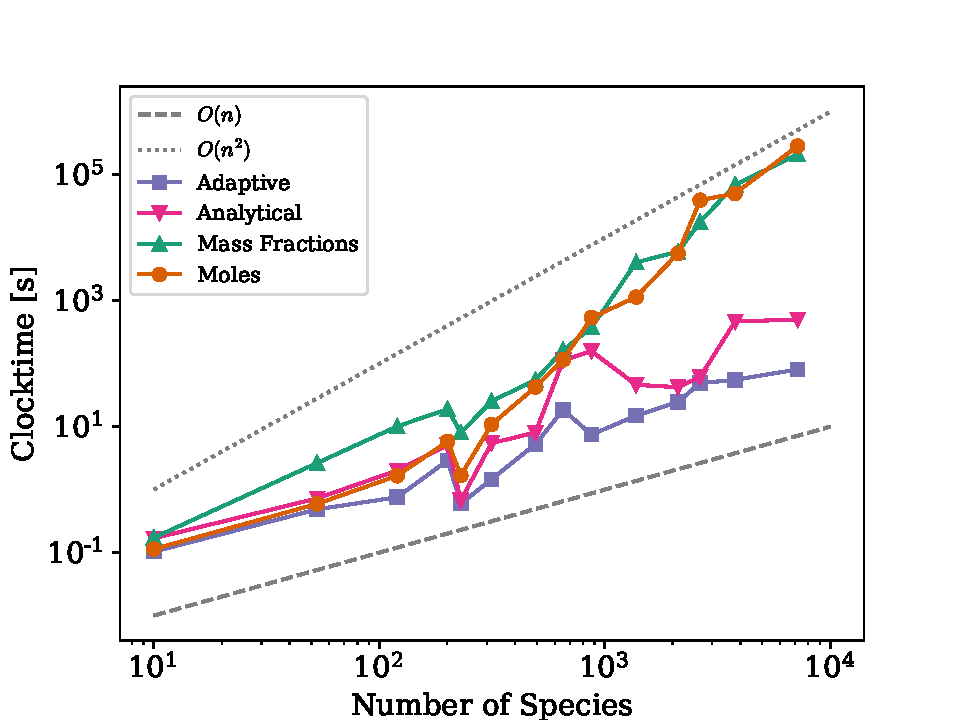
\includegraphics[width=0.49\textwidth]{figures/Clocktime-Nspecies-pressure_problem.pdf}
\caption{Clock time as a function of the number of species for preconditioned and non-preconditioned ideal gas constant-pressure systems.
The lines indicate linear and quadratic increases in time.}
\label{f:clocktime-nspecies-pressure}
\end{figure}

\begin{figure}[htb]
\centering
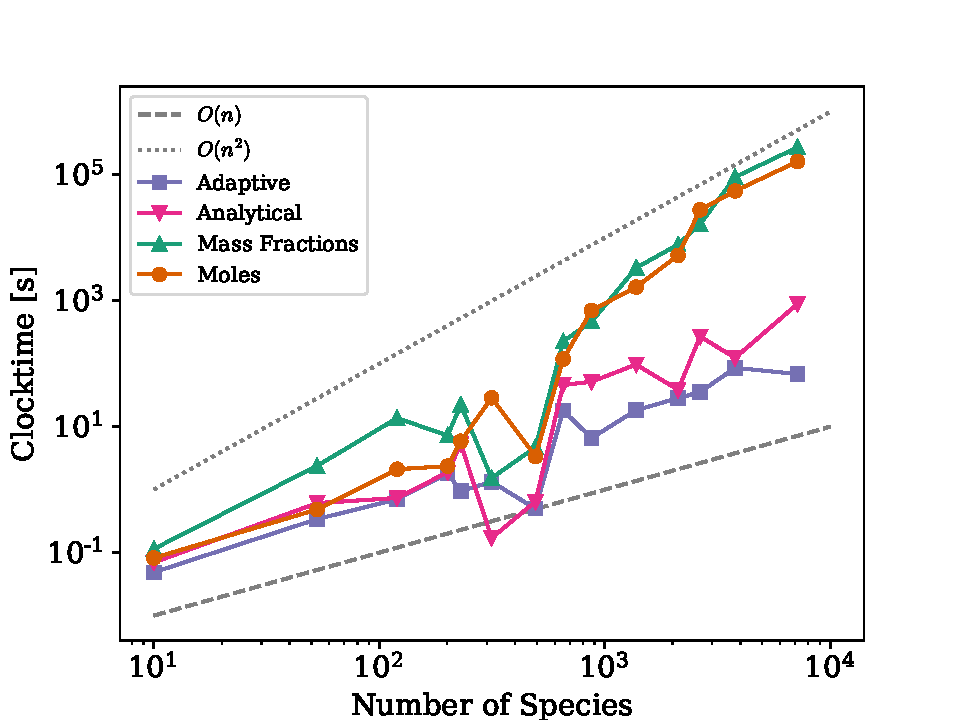
\includegraphics[width=0.49\textwidth]{figures/Clocktime-Nspecies-volume_problem.pdf}
\caption{Clock time as a function of the number of species for preconditioned and non-preconditioned ideal gas constant-volume systems.
The lines indicate linear and quadratic increases in time.}
\label{f:clocktime-nspecies-volume}
\end{figure}

Figures~\ref{f:clocktime-nspecies-pressure} and~\ref{f:clocktime-nspecies-volume} show the best-case wall-clock times of ignition simulations as a function of the number of species for constant-pressure and constant-volume reactors, respectively.
The preconditioned solver improves performance over direct solvers in clock time for all models, in both systems, in the best case (i.e., using the threshold value that leads to best performance).
For the largest models, we obtained speed-up of several orders of magnitude, and see the most benefit as the number of species increases.
The maximum speedups for both cases occur for the largest model considered, for 2-methyl-nonadecane model (with 7171 species)~\cite{sarathy_comprehensive_2011}, at factors of 2590 and 3978 for the constant-pressure and -volume cases, respectively.
In the worst cases, without using the proper threshold, the preconditioned solver reduces performance, by a factor of 0.78 with the hydrogen model~\cite{smith_gri-mech_1999} for constant pressure and 0.45 for the 2-butonane model~\cite{hemken_2017} for constant volume.
%Specifically, for the constant-pressure system, the maximum speed-up is 2590 for the 2-methyl-nonadecane model with 7171 species~\cite{sarathy_comprehensive_2011}, and the minimum speed-up is 0.78 with the hydrogen~\cite{smith_gri-mech_1999} model at 10 species over all thresholds. At best, the constant-volume problem shows a speed-up of 3978 for 2-methyl-nonadecane~\cite{sarathy_comprehensive_2011} and a worst case of 0.45 for the 2-Butonane~\cite{hemken_2017} model with 315 species over all thresholds.


The adaptive preconditioned solver also improves performance over a fully analytical preconditioned solver, up to a factor 13 for the 2-nethyl-nonadecane model~\cite{sarathy_comprehensive_2011}, and at worst by a factor of 0.05 for the 2-butonane model~\cite{hemken_2017} for the constant-volume problem.
For the constant-pressure problem, at best the adaptive preconditioning speeds up integration by a factor of 21 for the isooctane model~\cite{mehl_chemical_2009} and at worst by 0.24 for the methyl-5-decenoate model~\cite{herbinet_detailed_2010}.
Overall, the adaptive preconditioning offers significant improvement in performance for larger models, with a slight reduction in performance (at most just about half) for the smallest models.

The main factor behind the observed factors of speed-up appears to be the number of species in the model, with more acceleration for larger models.
However, the performance trends fluctuate based on model: for example, the DME-propane model at 122 species has average speed-ups of 13.5 and 6.55 for the constant-pressure and constant-volume problems, respectively.
The Jet-A model at 201 species has average speed-ups of 5.23 and 3.84.
The butane model has 230 species, similar to the number of species in the Jet-A model, but has average speed-ups of 12.1 and 20.3.
This deviation in performance with the Jet-A model suggests that there is more to performance gains than strictly the number of species.
In particular, Jet-A and DME-propane models have larger percentages of pressure-dependent reactions, which reduce speedup with the constant-volume problem.
In contrast, the butane model has lower percentages of these reaction types, and shows the opposite trend in speed-up.
These impacts are diminished for larger models because they have lower percentages of these reactions.


\begin{figure}[htb]
\centering
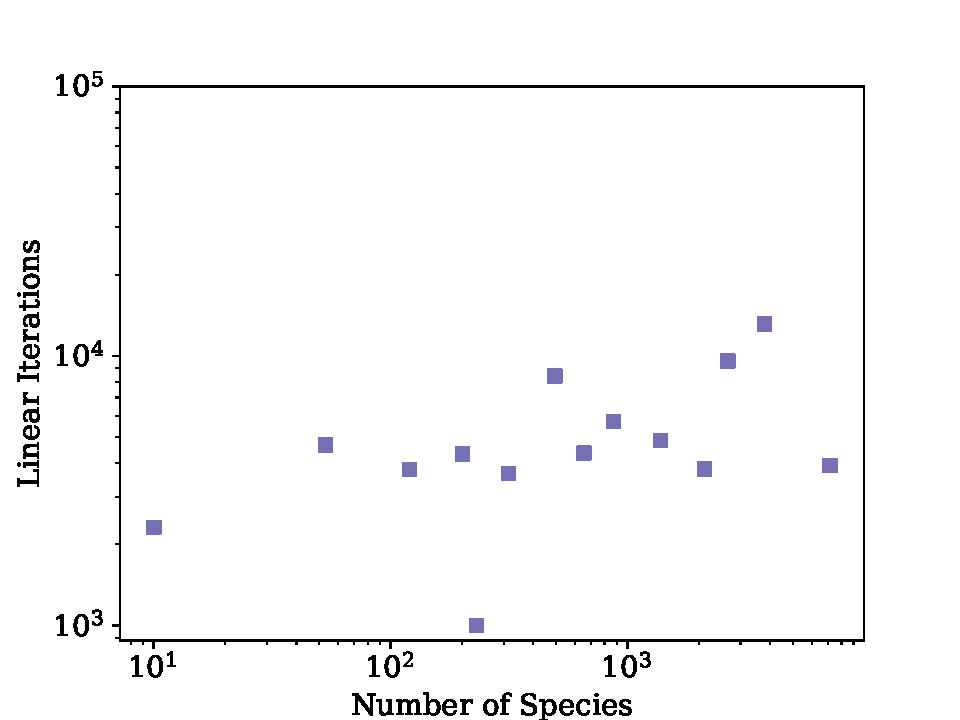
\includegraphics[width=0.49\textwidth]{figures/LinIters-Nspecies-pressure_problem.pdf}
\caption{Number of linear iterations as a function of the number of species.}
\label{fig:lin-iters-log}
\end{figure}

Performance increases are consistently accompanied by a reduction in the number of linear iterations taken by the preconditioned solvers.
Figure~\ref{fig:lin-iters-log} shows that the number of linear iterations remains roughly constant for the preconditioned method.
We see several spikes in the numbers of linear iterations, which are consistent with larger numbers of falloff and/or third-body reactions in a given model.
In particular, the Jet-A model has more of these reactions types than similar models, and consequently requires more linear iterations.

In contrast, the \textit{n}-heptane model has a large number third-body and falloff reactions, but it also has more total species, so the solution is less impacted by these reactions being present.
This trend is likewise carried through the rest of the results but more subtly because the impact is diluted by the number of species present.
For example, we see a valley in the clock time of the larger models (i.e., MD5D, MD \& \textit{n-}\ce{C7H16}, and \ce{C20H42}-2), which tracks well with the number of falloff/third-body and linear iterations in Fig.~\ref{fig:lin-iters-log}.
The performance likely depends on the number of these reaction types since these features are neglected in the formation of the preconditioner, suggesting that further improvements could be achieved by better-handling these reactions.

\begin{figure}[htb]
\centering
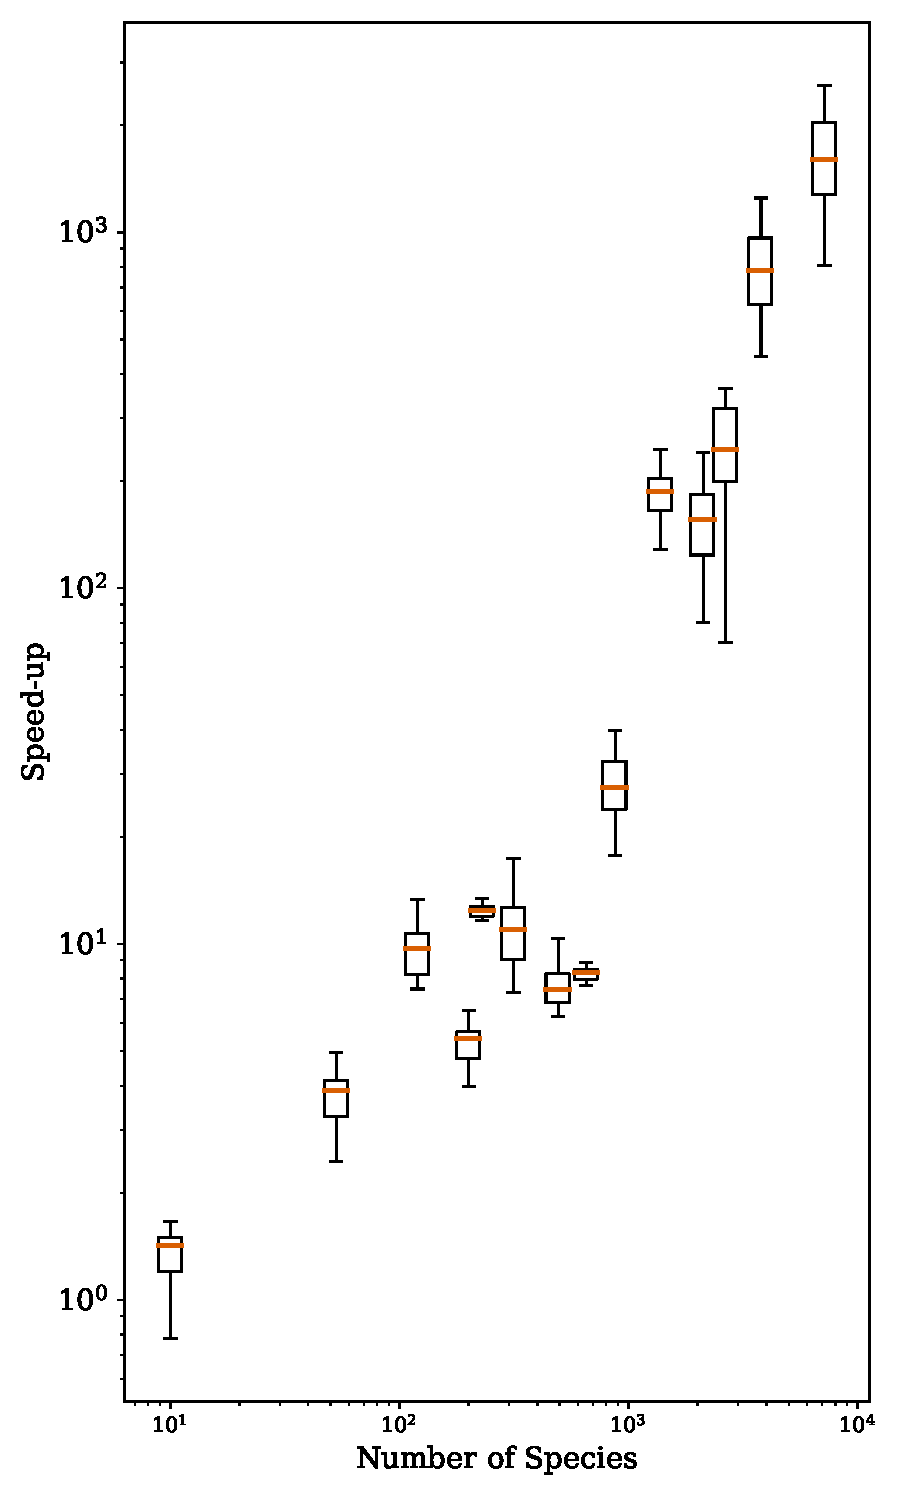
\includegraphics[width=0.49\textwidth]{figures/Threshold-BoxWhisker-pressure_problem.pdf}
\caption{Variation and median (orange line) speed-up of the preconditioned solver for the constant-pressure system with changes in threshold (over \numrange{1e-18}{1e-1} and 0).}
\label{fig:box_whisker}
\end{figure}


Figure~\ref{fig:box_whisker} shows the range of speed-up for the constant-pressure system as a function of the number of species, for all  threshold values considered.
The results for constant-volume are similar.
The threshold does impact the performance of the preconditioned solver, typically by a factor of two or three, with the maximum variation in speed-up being around an order of magnitude.
Furthermore, Figure~\ref{fig:box_whisker_iterations} shows the variation in total linear iterations as a function of model size, over all threshold values considered.
The number of linear iterations can vary substantially with different threshold values, although all models require similar numbers of iterations.

There are no definitive trends in optimal threshold based on model size or problem type.
The best and the worst thresholds for each model tend to be on opposite ends of the range of those tested, which suggests that choosing a threshold could be done effectively with a small number of tests.
However, regardless of the threshold value chosen, adaptive preconditioning achieves substantial performance gains in most cases.

\begin{figure}[htb]
\centering
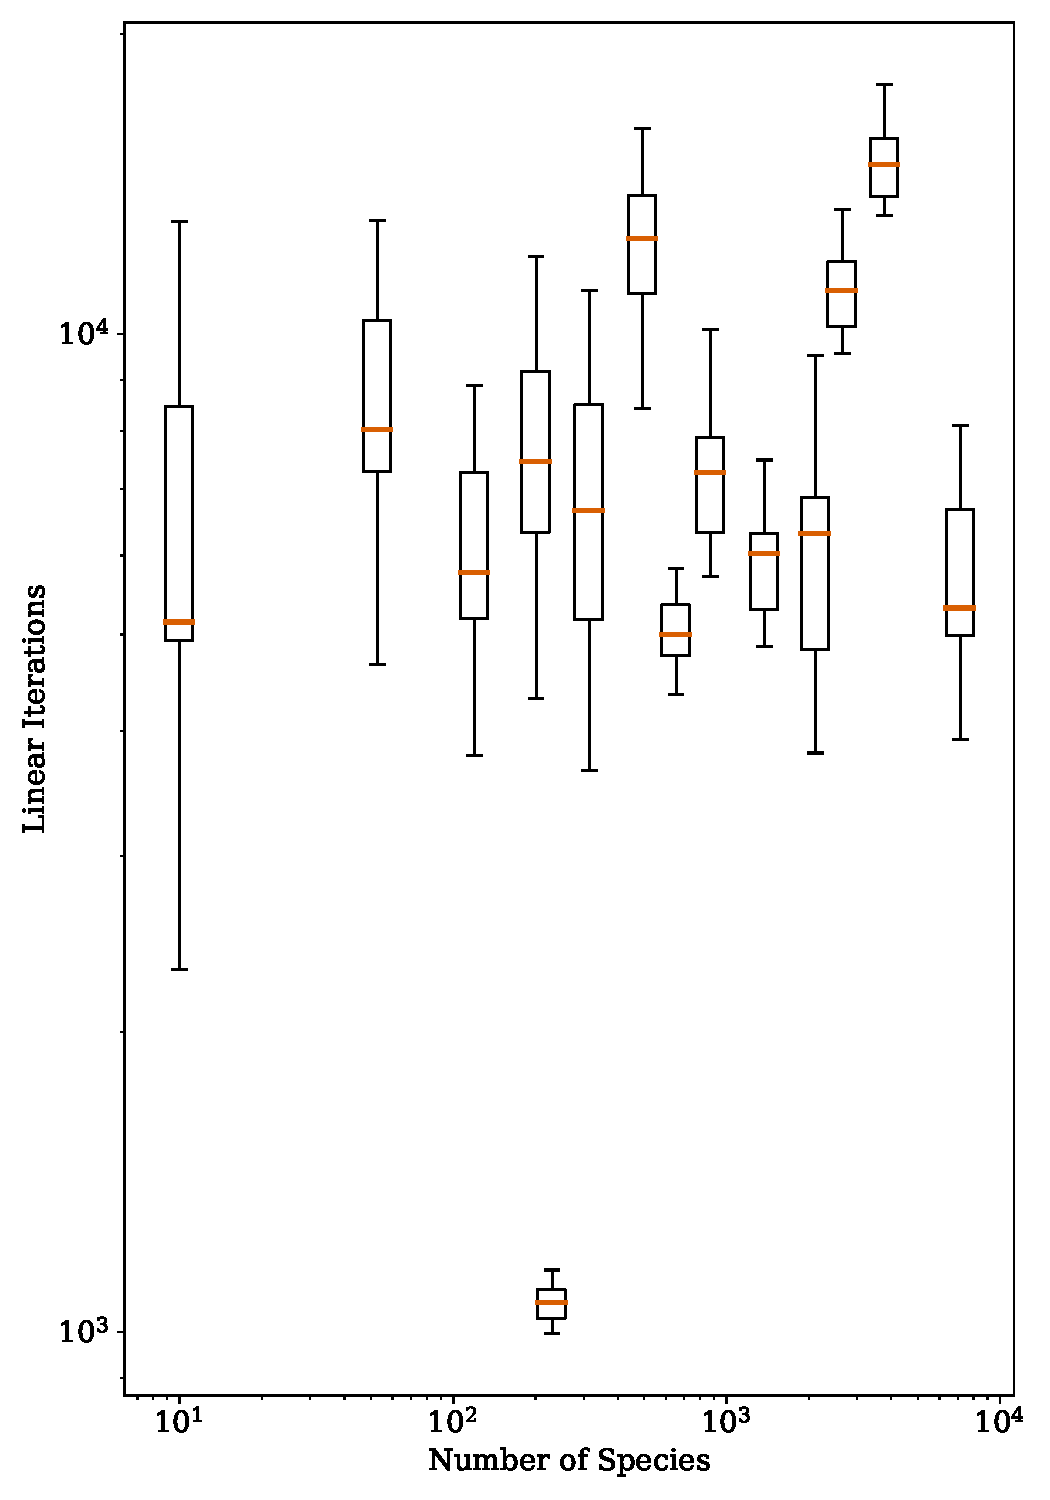
\includegraphics[width=0.49\textwidth]{figures/Iterations-BoxWhisker-pressure_problem.pdf}
\caption{Variation and median (orange line) normalized linear iterations of the preconditioned solver with changes in threshold (over \numrange{1e-18}{1e-1} and 0).}
\label{fig:box_whisker_iterations}
\end{figure}

\sectionOne{Conclusions}

In this work, we extended an adaptive preconditioning method for implicit ODE integrators.
Adaptive preconditioning neglects pressure dependence and third-body efficiencies when forming the Jacobian matrix,
uses finite differences for temperature derivatives, and prunes small preconditioner matrix elements based on a threshold value.
This also enables the use of sparse linear algebra operations.
We extended on the previously demonstrated adaptive preconditioning method to consider a state vector based on moles, allowing its use in more-general application such as constant-pressure reactors.
We tested this preconditioner on constant-pressure and constant-volume ideal-gas reactor simulations for kinetic models with a large range of species counts and over a range of threshold values.

In this application, the extended preconditioning method speeds-up performance by a factor of around 2 to nearly 4000 in comparison with direct solvers, for models with numbers of species from 10 to 7171.
The method improves performance over using a fully analytical Jacobian matrix as preconditioner by a factor of 0.24 to 21.1.

The potentially substantial performance gains of the solver strongly depend on the total number of species and the number of falloff\slash third-body reactions in the kinetic model.
These interactions directly influence the number of linear iterations required by the solver, which drives performance benefits.

Using a threshold to eliminate small Jacobian matrix elements improves performance by increasing Jacobian matrix sparsity.
However, there is no clear trend in optimal threshold, which makes determining appropriate values challenging.
Fortunately, the adaptive preconditioner offers substantial performance gains regardless of the specific threshold.
At most, the theshold value varies speedup by an order of magnitude, but typically by a factor of two or three.

Future work will explore the impact of threshold more thoroughly and how to balance sparsity with better-capturing third-body and pressure-dependent reactions in the semi-analytical Jacobian formulation.
In addition, we will investigate the specific causes for the performance improvement over using the fully analytical Jacobian matrix as preconditioner.
In addition, we will extend this method to support reactors with surface reactions and networks of reactors.

%\sectionOne{Acknowledgements \& References}

\acknowledgement{Acknowledgments} \addvspace{10pt}

This material is based upon work supported by the National Science Foundation under Grant Nos. 1931592 (OSU) and 1931391 (MIT).


\acknowledgement{Supplementary material} \addvspace{10pt}

The results and figures in this article can be reproduced using Cantera~\cite{cantera} and the testing package shared openly~\cite{testing_package}.
%Any plots not listed here can be easily produced with a combination of \cantera{} and the repository used for testing the updated features\footnote{github.com/anthony-walker/cantera}\footnote{github.com/anthony-walker/cantera-adaptive-testing}.
% -------------------------------------------------------------------- %
% -------------------------------------------------------------------- %
% -------------------------------------------------------------------- %

 \footnotesize
 \baselineskip 9pt

% -------------------------------------------------------------------- %
% -------------------------------------------------------------------- %
% -------------------------------------------------------------------- %

\bibliographystyle{symposium-template/pci.bst}
\bibliography{references.bib}

% -------------------------------------------------------------------- %
% -------------------------------------------------------------------- %
% -------------------------------------------------------------------- %

\newpage

\small
\baselineskip 10pt

% -------------------------------------------------------------------- %
% -------------------------------------------------------------------- %
% -------------------------------------------------------------------- %

% -------------------------------------------------------------------- %
% -------------------------------------------------------------------- %
% -------------------------------------------------------------------- %

\end{document}

% -------------------------------------------------------------------- %
% -------------------------------------------------------------------- %
% -------------------------------------------------------------------- %
